\cleartooddpage[\thispagestyle{empty}]
\chapter{Introduction}

  How much mass is contained within a given volume of space?
  Within a Galaxy?
  Within a Cluster of Galaxies?
  Within the observable universe?

  These questions have been asked repeatedly since the 1930s, but different measurements produce conflicting answers.
  Observing cosmological features like the cosmic microwave background, the distribution of galaxies, and gravitational lensing around galaxy clusters results in a larger mass, while observing the quantity of light produced results in a smaller mass.
  The cosmic micrwave background's spectrum is only well fit if there is much more mass present in the universe than is currently interacting with light.
  Galaxies are observed to rotate quite fast, much faster than their bayronic mass alone would allow.
  In addition, galaxy clusters have two clouds of mass, one of hydrogen gas observable via X-Ray observations, another observable via the gravitational lensing of visible light.
  Collisions between two clusters cause these two clouds to pass through each other, dragging and slowing each other down at different rates.
  The differences in drag hints that the gravitationally-lensed mass has a smaller cross-section than the hydrogen gas cross-section.
  
  All of this heavily implies that there is missing mass, missing \textit{stuff}, unaccounted for by the existing model of physics and our universe.
  As this mass prefers to only interact gravitationally and seemingly ignores the electromagnetic spectrum, it has earned the (in)conspicuous title of Dark Matter.

\section{Motivation}
  This thesis will demonstrate that, by detecting gamma-rays from the Galactic Center with the VERITAS observatory, a search for a Dark Matter can be conducted.
  Dark Matter is proposed to be a particle that annihilates with itself into standard model particles.
  If Dark Matter particles form a spherical cloud (referred to as a halo) around the center of our galaxy, and if the annihliation of these particles produces (either directly or through secondary interactions) a detectable quantity of gamma rays, the density profile of this Dark Matter halo can be measured.
  If instead the gamma-ray flux is below detection limits, then knowledge of the observatory's sensitivity can place an upper limit on the cross-section of the dark matter particle.

\section{Dark Matter}

  % WMAP: 4.6% energy from baryonic matter, 24% energy from cold dark matter
  From measuring the cosmic microwave background, the WMAP satellite found that Dark Matter makes up 24\% of the energy of the universe~\cite{pdg_2012}, thus understanding the nature of Dark Matter is fundamental to understanding our universe.
  It is currently believed that Dark Matter is a particle, not included in the standard model of particle physics.
  As many particle models either predict it to either a) couple weakly to other particles, b) interact via the Weak force, or c) both, it is referred to as a Weakly Interacting Massive Particle, or WIMP.

  From both cosmology and particle physics, the WIMP is predicted to have a mass in the range of GeV to TeV, and a velocity-averaged self-annihilation cross-section of around \nicetilde{}\SI{3e-26}{cm${}^3$s${}^{-1}$}.
  WIMPs may directly annihilate or decay into gamma rays, or they may first produce quarks or leptons, which would then produce gamma rays through secondary interactions.
  These gamma rays would then have energies similar to the original WIMP mass, around the TeV scale.
  This potential for WIMP Dark Matter to produce TeV gamma rays makes it an attractive science target for gamma-ray observatories like VERITAS.

  Then, the question becomes, where should we point our gamma-ray observatories?
  From gravitational and optical measurements, it is well documented that halos of Dark Matter augment the gravitational wells of most dwarf galaxies, regular galaxies, and galaxy clusters.
  Dwarf galaxies tend to have fewer background gamma-ray sources, but also have lower quantities of Dark Matter, making them weaker sources of dark matter gamma rays.
  Galaxy Clusters, while more massive (and thus more emissive), have a non-negligable redshift, which introduces more model parameters.
  The Galactic Center, on the other hand, possesses higher densities of Dark Matter mass than any dwarf galaxy, while also being closer than any dwarf galaxy, making it an excellent target for gamma-ray Dark Matter searches.


\section{Galactic Center and Gamma Rays}

  At the center of our galaxy there is a supermassive black hole, with a mass of \SI{4e6}{\Msol{}}~\cite{sgra_massdist}.
  As Dark Matter appears to accompany most Baryonic gravitational wells, it is expected that there is a halo of dark matter particles at the Galactic Center.
  Studying this halo is difficult, however, as our galaxy's large graviational well has accreted a large amount of dust, as well as there being a large number of stars and supernova remntants nearby.

  % see Dropbox/Research/Thesis/images/GalacticCenterInRadio.key for figure construction
  \begin{figure}[ht]
    \centering
    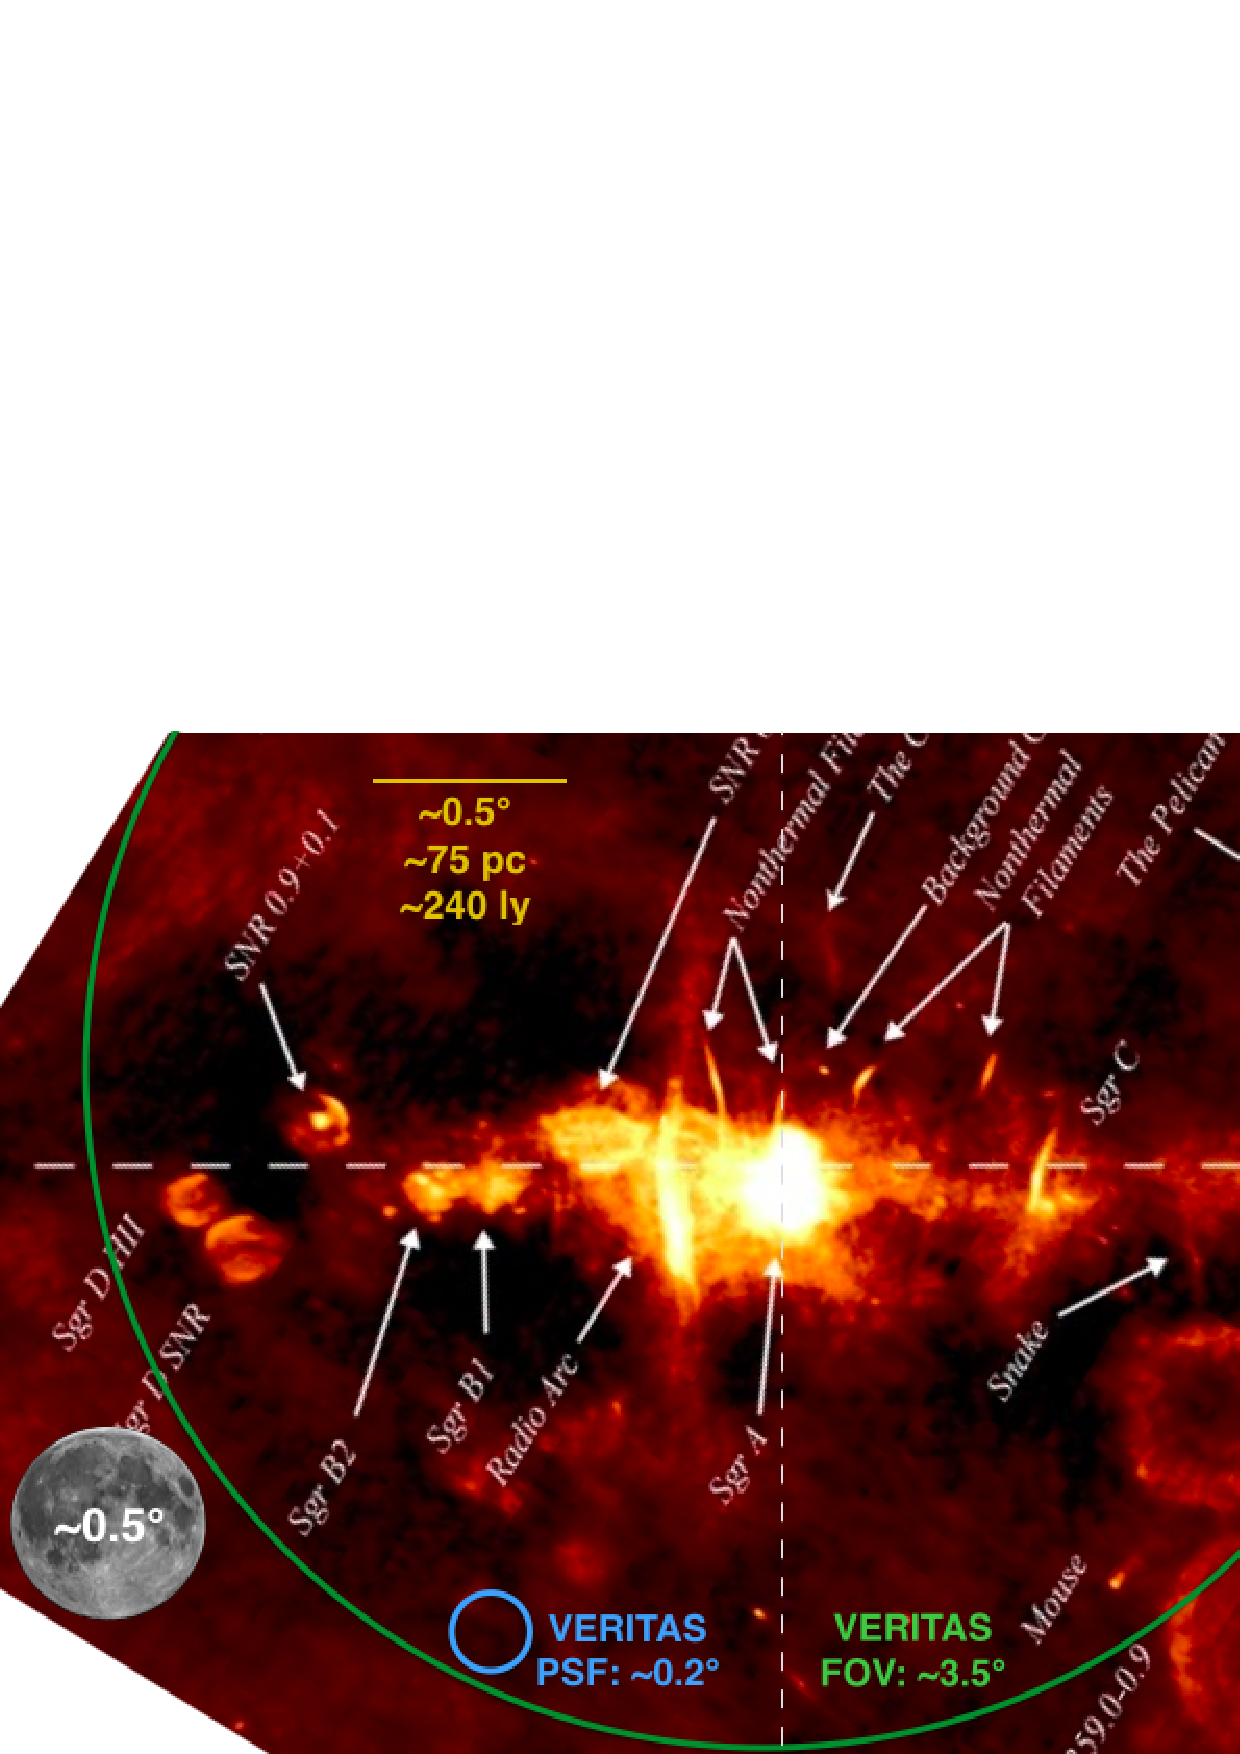
\includegraphics[width=0.95\textwidth]{images/GalacticCenterInRadio/GalacticCenterInRadio.pdf}
    \caption[Galactic Center in Radio]{
      The center of our galaxy, viewed at a radio wavelength of $\lambda=90\text{cm}$.
      The horizontal dashed line roughly represents the galactic plane, where the intersection of the dashed lines indicates the center of our galaxy.
      Supernova remnants and dust are visible in the view.
      The VERITAS field of view, the VERITAS point source spread (68\% containment), and the moon are shown for angular scale.
      Radio flux image is from Ref. \cite{galactic_center_in_radio}.}
    \label{fig_gc_radio}
  \end{figure}

  The dust, supernova remnants, and the Galactic Center itself all emit gamma rays, making detection of a dark matter halo difficult.
  The dust operates as a collision target for high-energy protons from other galaxies, whose interactions produce $\pi_0$ particles, which then decay into gamma rays.
  These dust-induced gamma rays are collectivly referred to as Diffuse Emission, and appear as a disk of gamma rays along the galactic plane.
  The supernova remnants accelerate electrons and protons outwards, which then shock into the surrounding dust and gas, producing gamma rays.
  The black hole at the Galactic Center also produces gamma rays in a point-like shape (point-like relative to the other sources), though the mechanism by which it does this is not well understood~\cite{gal_cent_still_undetermined}.

  These effects all obscure the target of this analysis, the gamma ray emission from a dark matter halo.
  This spherically-symmetric halo of gamma rays would surround the Galactic Center, decreasing in intensity the further from the center.
  The halo's spectrum would also be different from the surrounding diffuse emission.

  Once these gamma rays have been emitted, they would travel to Earth, where humans can detect them.
  This is done by using a telescope to observe the particle shower that occurs when each gamma ray hits the Earth's atmosphere.
  The VERITAS telescope has been observing gamma rays from the Galactic Center for several years.
  The data from these observations are used in this analysis.


\section{Halo Analysis}
  After several years of operation, VERITAS has accumulated \SI{108}{hours} of Galactic Center data.
  To analyze these observations, an unbinned likelihood analysis is used.
  With this analysis, the Galactic Center region is modeled with nine different dark matter halos, and the statistical existance of each halo can be calculated.
  For the spatial shape of the dark matter halo, a cuspy Einasto profile is chosen.
  For the spectral shape, only the $b\bar{b}$ annihilation channel is used.
  Each of the nine dark matter halos is modeled with a different dark matter mass $m_{\chi}$, which changes the spectrum of gamma rays produced in each $\chi\chi$ annihilation.
  
  From this analysis, no dark matter signal was found at any of these masses.
  With this null result, the next step is to calculate the upper limit on the velocity-averaged cross-section of this WIMP.
  From these upper limits, new limits can be placed on the WIMP velocity-averaged cross-section at \SI{100}{TeV}.


